\documentclass[11pt, a4paper, twoside]{article}   	% use "amsart" instead of "article" for AMSLaTeX format

\usepackage{geometry}                		% See geometry.pdf to learn the layout options. There are lots.
\usepackage{pdfpages}
\usepackage{caption}
\usepackage{minted}
\usepackage[german]{babel}			% this end the next are needed for german umlaute
\usepackage[utf8]{inputenc}
\usepackage{color}
\usepackage{graphicx}
\usepackage{titlesec}
\usepackage{fancyhdr}
\usepackage{lastpage}
\usepackage{hyperref}
% http://www.artofproblemsolving.com/wiki/index.php/LaTeX:Symbols#Operators
% =============================================
% Layout & Colors
% =============================================
\geometry{
   a4paper,
   total={210mm,297mm},
   left=20mm,
   right=20mm,
   top=20mm,
   bottom=30mm
 }	

\definecolor{myred}{rgb}{0.7,0.3,0.4}
\definecolor{mygreen}{rgb}{0,0.6,0}
\definecolor{mygray}{rgb}{0.5,0.5,0.5}
\definecolor{mymauve}{rgb}{0.58,0,0.82}

\setcounter{secnumdepth}{4}


% the default java directory structure and the main packages
\newcommand{\dotNetRoot}{../source/dot-net}
\newcommand{\javaRoot}{../source/java}
\newcommand{\imagesRoot}{images}
% the default subsection headers
\newcommand{\ideaSection}{Lösungsidee}
\newcommand{\sourceSection}{Source-Code}
\newcommand{\testSection}{Tests}

% =============================================
% Code Settings
% =============================================
\newenvironment{code}{\captionsetup{type=listing}}{}
\newmintedfile[javaSourceFile]{java}{
	linenos=true, 
	frame=single, 
	breaklines=true, 
	tabsize=2,
	numbersep=5pt,
	xleftmargin=10pt,
	baselinestretch=1,
	fontsize=\footnotesize
}
\newmintinline[inlineJava]{java}{}
\newminted[javaSource]{java}{
	breaklines=true, 
	tabsize=2,
	autogobble=true,
	breakautoindent=false
}
\newmintedfile[xmlSourceFile]{xml}{
	linenos=true, 
	frame=single, 
	breaklines=true, 
	tabsize=2,
	numbersep=5pt,
	xleftmargin=10pt,
	baselinestretch=1,
	fontsize=\footnotesize
}
\newmintedfile[propertiesFile]{properties}{
	linenos=true, 
	frame=single, 
	breaklines=true, 
	tabsize=2,
	numbersep=5pt,
	xleftmargin=10pt,
	baselinestretch=1,
	fontsize=\footnotesize
}
% =============================================
% Page Style, Footers & Headers, Title
% =============================================
\title{Übung 3}
\author{Thomas Herzog}

\lhead{Übung 3}
\chead{}
\rhead{
\includegraphics[scale=0.10]{FHO_Logo_Students.jpg}}

\lfoot{S1310307011}
\cfoot{}
\rfoot{ \thepage / \pageref{LastPage} }
\renewcommand{\footrulewidth}{0.4pt}
% =============================================
% D O C U M E N T     C O N T E N T
% =============================================
\pagestyle{fancy}
\begin{document}
\setlength{\headheight}{15mm}
%\includepdf[pages={1-3}]{Swe4xA05-BB.pdf}
{\color{myred}
	\section
		{UFO (Ultimate - Festival - Organizer)}
}
Folgende Dokumentation stellt die Gesamtdokumentation der aufbauenden Übung UFO dar, die im Zuge der Realisierung iterativ über die drei Ausbaustufen hinweg erweitert wird. \\

\subsection{Ausbaustufe 1 (ADO.NET)}
Folgender Teil dokumentiert die erste Ausbaustufe der aufbauenden Übung UFO. In diesem Teil wird die Persistenz Schicht in .NET unter Hilfenahme von ADO.NET implementiert. Aufgrund der Analyse der Gesamtaufgabenstellung wurde entschieden das vorerst nur die Persistenz Schicht an sich, also INSERT, UPDATE, DELETE der einzelnen Entitäten realisiert wird, da die Geschäftslogik erst bei der Realisierung der Administration und des Webzugriffs endgültig feststehen wird. \\\\
Im Zuge der Realisierung des Webzugriffs wird auch der Web-Service implementiert werden müssen, der die Daten der Web Applikation zur Verfügung stellt. Dieser soll die Daten bereits gefiltert und strukturiert zur Verfügung stellen, daher besteht eine gewisse Abhängigkeit zwischen dem Web-Service und der Web Applikation sowie auch der Client Administration.\\\\
Daher werden die Web-Service Implementierung und die Administration die eigentliche Geschäftslogik enthalten, die 
in einer Transaktion abgearbeitet und im wesentlichen aus den logischen Prüfungen gegen die Datenbank bestehen wird sowie der Speicherung und Löschung von Entitäten über die Administration. Die einzelnen Datenabfragen, die benötigt werden können einfach hinzugefügt werden.

\subsubsection{Systemaufbau}
Folgend ist der Systemaufbau der Persistenz Schicht dokumentiert.\\\\
Die folgende Auflistung illustriert die Projektstruktur der Persistenz Schicht:
\begin{enumerate}
	\item\emph{UFO.Server.Data.Api}\\
	 Dieses Projekt enthält die Spezifikation der Persistenz Schicht in Form von 	      Interfaces, abstrakten Klassen, Exceptions und den Entitäten, die wie bei einem ORM-Mapper DB unabhängig sein sollen (sofern möglich).
	 \item\emph{UFO.Server.Data.MySql}\\
	 Dieses Projekt enthält die MySql spezifische Implementierung der Persistenz Schicht.
	 \item\emph{UFO.Server.Test.Data.MySql}\\
	 Dieses Projekt enthält die MySql spezifischen Tests der Persistenz Schicht.
	 \item\emph{UFO.Common.Util}\\
	 Dieses Projekt enthält die Utlities für die UFO Infrastruktur in .NET, die nicht spezifisch einen Systemteil zuzuordnen sind.
	 \item\emph{ufo-data-generator}\\
	 Ein kleines Java Projekt welches eine Java Main Klasse enthält und die benötigen Ressourcen um das Testdatenskript zu erstellen. Hierzu wurde \emph{freemarker} verwendet.
\end{enumerate}
Alle .NET Systemteile werden unter dem Namensraum \emph{UFO.*} zusammengefasst.

\newpage
Die folgende Auflistung illustriert die verwendeten Technologien und Frameworks:
\begin{enumerate}
	\item\emph{MySql}\\
	Es wird eine MySql Datenbank verwendet, die Open-Source ist und eine Integration in .NET besitzt.
	\item\emph{NUNIT}\\
	Als Test-Framework wird NUNIT verwendet, da es mehr Funktionalität mitbringt als das Standard Test-Framework integriert in .NET.
	\item\emph{ADO.NET}\\
	Als Persistenz Provider wird wie gewünnscht ADO.NET und kein ORM Mapper verwendet.
	\item\emph{freemarker}\\
	Template-Engine in Java mit der das Testdaten SQL Skript erstellt wird.
\end{enumerate}

\newpage
\subsubsection{Datenbank}
Es wurde als Datenbank MySql und Moderlierungstool MySql Workbench gewählt, da diese Datenbank erstens Open-Source, zweitens eine gute .NET Integration vorhanden ist sowie drittens bereits Erfahrungen mit dieser Datenbank vorhanden waren.\\\\
Es wurden folgende Skripten generiert die einerseits für die Tests und andererseits für die Generierung der Testdaten genutzt werden. Diese Skripten befinden sich im Projekt \emph{UFO.Server.Data.MySql/Resources}.\\
\begin{enumerate}
	\item\emph{createDatabase.sql}\\
	Ein vollständiges Skript für das Anlegen der Datenbank mit allen Constraints und verwendeten Triggern.
	\item\emph{deleteDatabase.sql}\\
	Ein Skript welches alle Einträge in der Datenbank löscht.
	\item\emph{dropDatabase.sql}\\
	Ein Skript für das Droppen der Datenbank UFO.
	\item\emph{createTestData.sql}\\
	Ein Skript welches die Testdaten generiert.
\end{enumerate}
\ \\
Die Testdaten wurden mit einer Java Applikation mit Hilfe von \emph{Freemarker} erstellt, welches eine Template Engine darstellt. Die Daten werden von \emph{*.csv} Dateien zur Verfügung gestellt und anschließend über eine Java Konsolen Applikation verarbeitet. Diese Applikation liest die Daten ein, verpackt diese in Pojos, generiert dynamische Daten, wie z.B.: die Aufführungen mit den Aufführungszeiten und stellt diese Daten einem Template zur Verfügung.

\newpage
Das folgende ER-Diagramm illustriert das implementierte Datenbank Schema.
\begin{figure}[h]
	\centering
	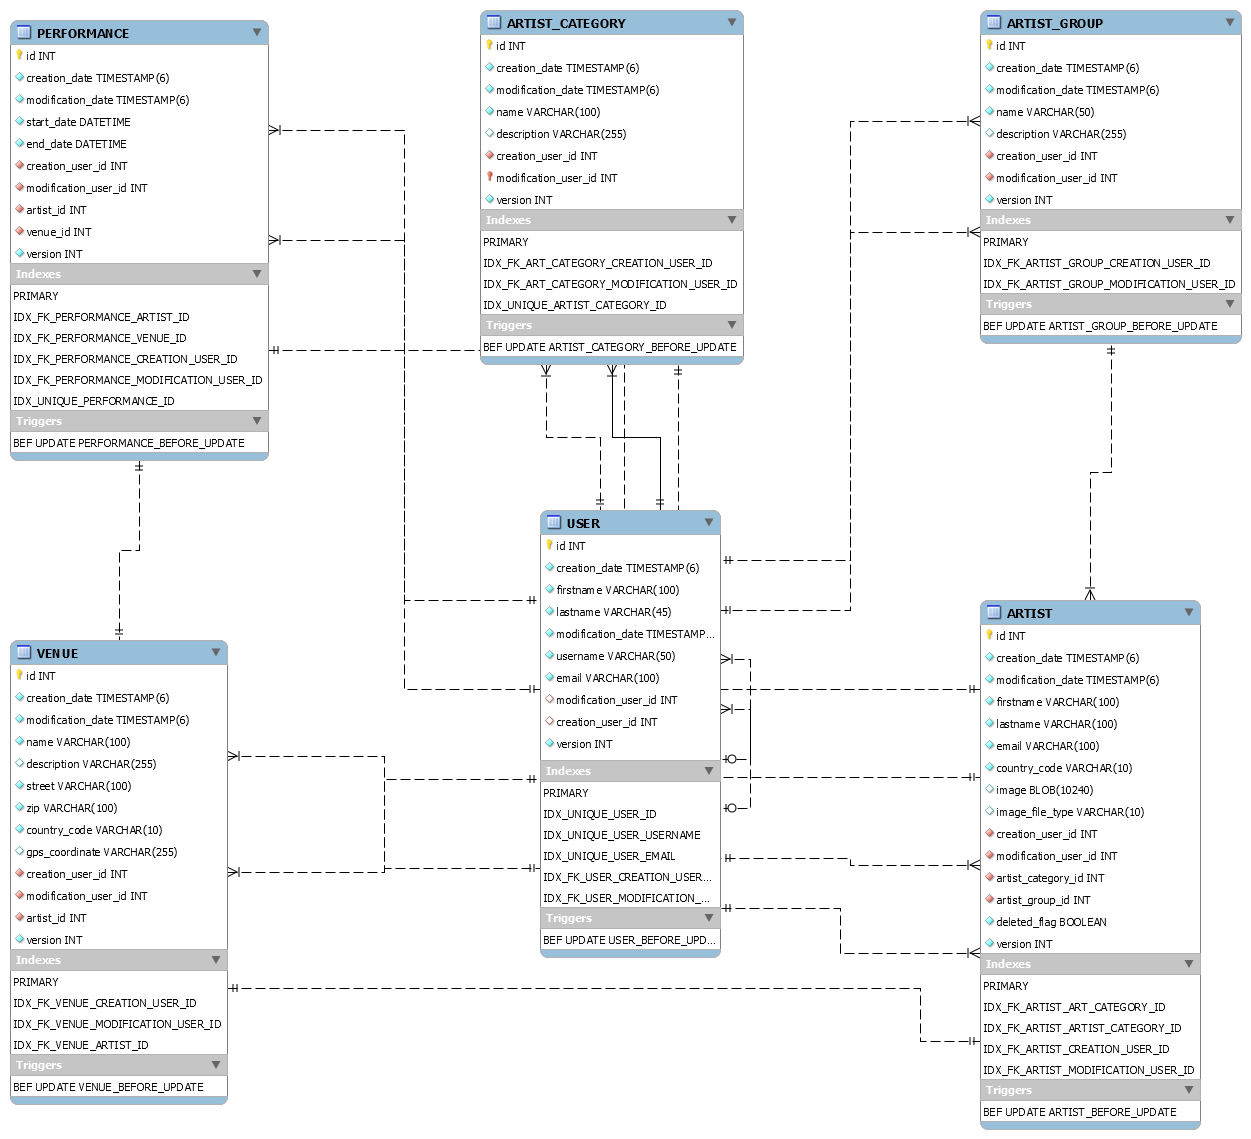
\includegraphics[scale=0.35]{\imagesRoot/er_diagram.PNG}
	\caption
	{ER-Diagramm des Schema 'UFO'}
\end{figure}
\ \\
Auf jeder Entität wurde eine Spalte für die Versionierung eingeführt (MySqlDbType.LONG), die über einen Update-Trigger bei jedem Update um eins erhöht wird sowie auch das Modifizierungsdatum. Ein ganzzahliger Datentyp erschient hier mehr sinnvoll, da es hier mit Sicherheit keine Kollisionen geben kann, nicht so wie bei einem Zeit Datentyp.\\\\
Ebenso halten alle Entitäten eine Referenz auf den Benutzer der Sie erstellt sowie zuletzt modifiziert hat. Dies dient der Nachverfolgbarkeit von Änderungen, zumindest wer zuletzt eine Änderung vorgenommen hat.

\newpage
\subsubsection{Klassenhierarchien}
Folgend sind die Klassenhierarchien der implementierten Klassen und Interfaces dokumentiert.\\

\textbf{\emph{IDao}}\\
Folgendes Klassendiagramm zeigt die Hierarchie des Interfaces \emph{IDao}, das der Basistyp für alle implementierten DAO Interfaces dient, da es bereits alle Basisaktionen auf eine Entität definiert.
\begin{figure}[h]
	\centering
	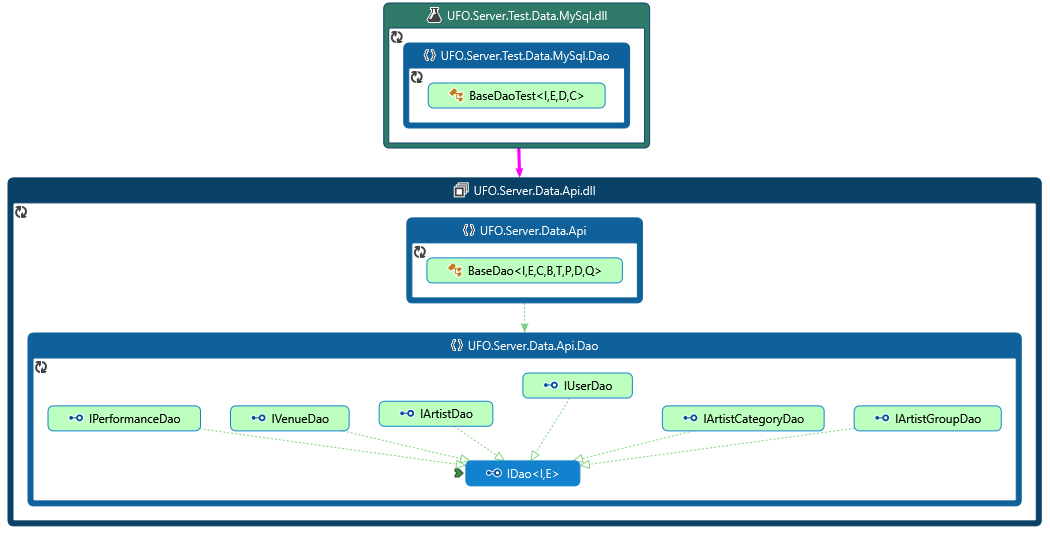
\includegraphics[scale=1]{\imagesRoot/idao_map.PNG}
	\caption
	{Klassenhierarchie IDao Interface}
\end{figure}
\ \\
Die Basisklasse  \emph{BaseDao} implementiert alle Methoden, die in \emph{IDao} definiert wurden für alle implementieren Entitäten sofern sie \emph{IEntity} implementieren. Dieser generische und abstrakte Ansatz erlaubt es dass die Basisfunktionalität eines DAOs nur einmal für alle Entitätstypen, die \emph{IEntity} implementieren, implementiert werden musste.\\\\
Die \emph{DAOs} für die einzelnen Entitäten werden zukünftig Methoden implementieren, die spezifische Datenbankabfragen realisieren, die z.B.: eine komplexe \emph{where caluse} aufweisen, die ihrerseits wieder einen Teil der Geschäftslogik enthält, welche noch nicht vollständig bekannt ist.

\newpage
\textbf{\emph{IEntity}}\\
Folgendes Klassendiagramm illustriert die Klassenhierarchie des Interfaces \emph{IEntity}, welches den Basistyp für alle Entitäten darstellt.
\begin{figure}[h]
	\centering
	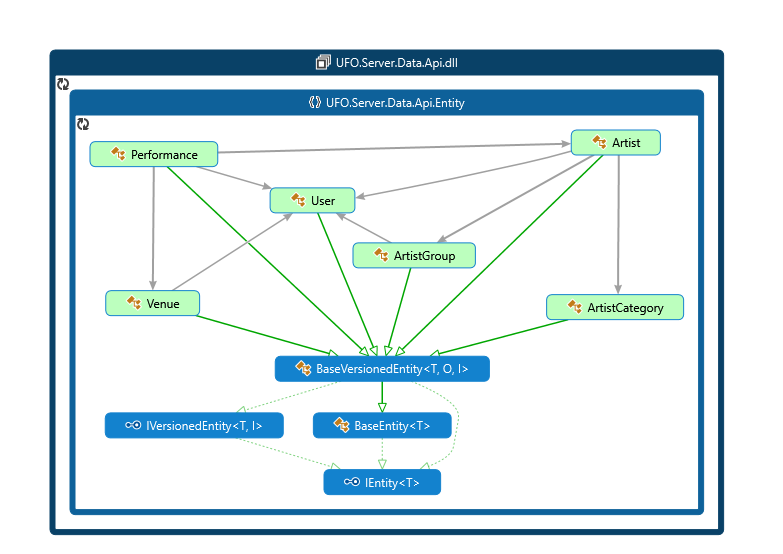
\includegraphics[scale=1]{\imagesRoot/ientity_map.PNG}
	\caption
	{Klassenhierarchie IEntity Interface}
\end{figure}
\ \\
Es wurden Basisentitäten eingeführt, welche eine Basisstruktur definieren dies sich Entitäten unterwerfen müssen wenn sie von diesen Klassen ableiten. Somit wird eine konsistente Struktur der Entitäten bzw. deren Tabellenrepräsentation gewährleistet.\\\\
Die Aufteilung von \emph{IEntity} und \emph{IVersionedEntity} wurde eingeführt, da eine Entität nicht zwangsweise versionierbar sein muss. Ebenso wurde mit den abstrakten Klassen verfahren, die jetzt eine Hierarchie abbilden anstatt die gesamte Funktionalität in eine abstrakte Klasse zu packen.

\newpage 
\textbf{\emph{IEntityHelper}}\\
Folgendes Klassendiagramm illustriert die Klassenhierarchie des Interfaces \emph{IEntityHelper} welches die Utility Methoden für das generieren von Entitäten definiert.
\begin{figure}[h]
	\centering
	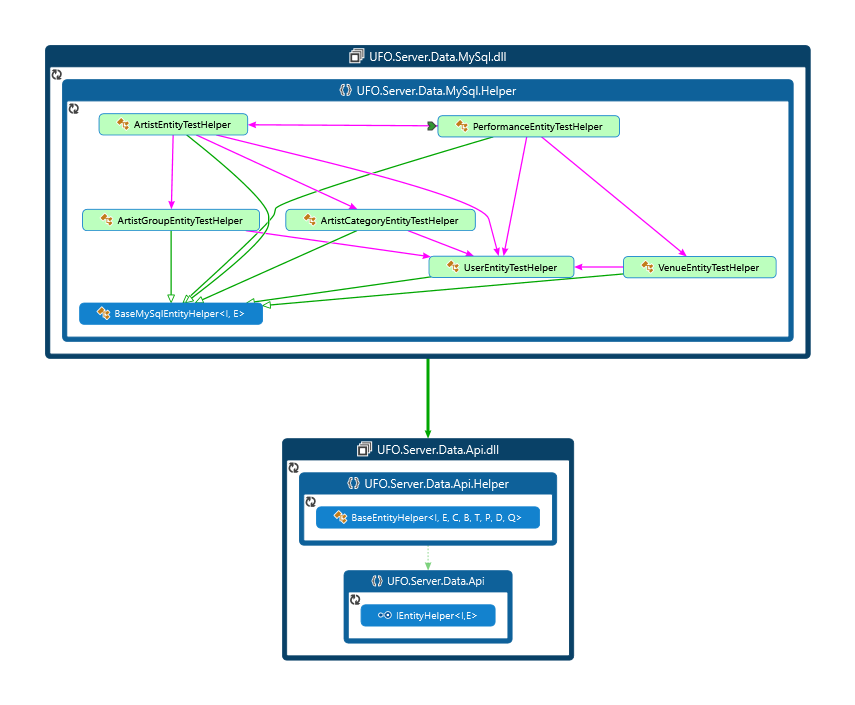
\includegraphics[scale=1]{\imagesRoot/ientityhelper_map.PNG}
	\caption
	{Klassenhierarchie IEntityHelper Interface}
\end{figure}
\ \\
Dieses Interface und dessen Implementierungen diesen als Hilfestellung für die Test und die Generierung von Testdaten über die Entitäten Modelle. Die abstrakte Basisklasse \emph{BaseEntityHelper} implementiert einige der Interface Methoden und stellt eine Persistenzprovider unabhängige Implementierung für das einfache Speichern von Entitäten zur Verfügung. Diese Hilfsklassen entstanden aufgrund der generischen Testklasse \emph{BaseDaoTest}, die die Entitäten nicht erzeugen kann und daher diese von außen zur Verfügung gestellt werden müssen.

\newpage
\textbf{\emph{BaseCommandBuilder}}\\
Folgendes Klassendiagramm illustriert die abstrakte Klasse \emph{BaseCommandBuilder} die das Handling mit einen \emph{DbCommand} beinhaltet. 
\begin{figure}[h]
	\centering
	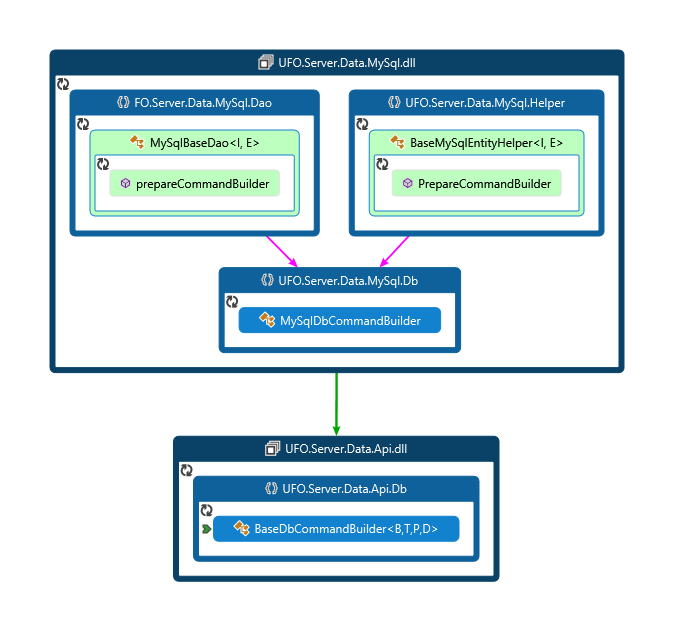
\includegraphics[scale=1]{\imagesRoot/basecommandbuilder_map.PNG}
	\caption
	{Klassenhierarchie der abstrakte Klasse BaseCommandBuilder}
\end{figure}
\ \\
Um zu vermeiden sich mit dem Code des Erstellens, Modifizierens und Verwerfens eines \emph{DbCommand}, in unserem Fall ein \emph{MySqlDbCommand}, herumschlagen zu müssen, wurde beschlossen eine Hilfsklasse einzuführen, die uns dieses Handling mit einem \emph{DbCommand} abnimmt.
Da sich hier eine Fluent-API gut anwenden lässt, wurde diese Funktionalität in Form eines Builder abgebildet.

\newpage
\textbf{\emph{IQueryCreator}}\\
Folgendes Klassendiagramm illustriert das Interface \emph{IQueryCreator}, die die Datenbank spezifischen Statements enthält.
\begin{figure}[h]
	\centering
	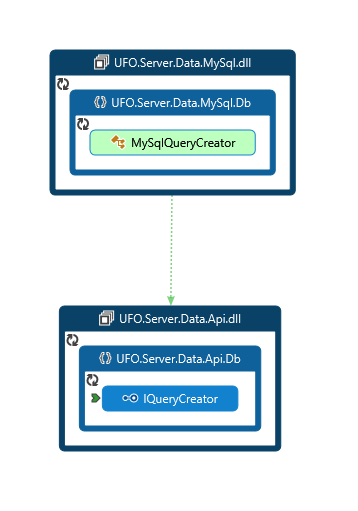
\includegraphics[scale=1]{\imagesRoot/iquerycreator_map.PNG}
	\caption
	{Klassenhierarchie des Interface \emph{IQueryCreator}}
\end{figure}
\ \\
Diese Interface abstrahiert die Datenbank spezifischen Statements von der Klient Logik. Ebenso erlaubt sie es alle Statements in einem Interface abzubilden und diese an einer Stelle pro Entität zu bündeln. 

\newpage
\subsubsection{Hilfsklassen}
Im folgenden werden die Hilfsklassen beschrieben, die eingeführt wurden um sich wiederholende und daher immer wiederkehrende Funktionalitäten zu kapseln und zentral zur Verfügung zu stellen.\\\\

\textbf{\emph{EntityMetamodel}}\\
Diese Klasse löst die Meta-Informationen eines \emph{IEntity} Typs auf und stellt diese aufbereitet nach außen zur Verfügung. Da sich diese Daten zur Laufzeit nicht ändern und daher nur einmalig erzeugt werden sollen, wird eine Factory \emph{EntityMetamodelFactory} eingeführt, die  das Caching der \emph{EntityMetamodel} übernimmt.\\\\

\textbf{\emph{EntityBuilder}}\\
Diese Klasse wurde eingeführt um die Transformation von den Entitäten zur Datenbank und visa versa zu unterstützen, wobei hier einerseits die Werte der Properties, die auf die Datenbank serialisierbar sind, ausgelesen und auf den Property gemapped werden und andererseits die De-Serialisierung vom \emph{IDataReader} zu einer Entität.\\\\

\textbf{\emph{IDbTypeResolver}}\\
Implementierungen dieses Interface lösen einen C\# Typ in einen korrespondierenden Datenbank spezifischen Typ auf.\\\\

\textbf{\emph{DbConnectionFactory}}\\\\
Diese Klasse erstellt und verwaltet die verwendeten \emph{DbConnection} Instanzen. Der Typ der zu verwendenden \emph{DbConnection} wird über die \emph{App.config} definiert, sowie der \emph{ConnectionString}.

\newpage
\subsubsection{Tests}
Die Tests bestehen aus einer einzigen Testklasse, die das \emph{IDao} Interface bzw. die dessen Ableitungen bzw. dessen Implementierungen, die zurzeit nur aus der Implementierung in \emph{BaseDao} bestehen. Also die Basis Dao Funktionalitäten beinhalten wie.\\
\begin{enumerate}
	\item\emph{dao.ById // Throws Exception}
	\item\emph{dao.Find // Returns null}
	\item\emph{dao.Update}
	\item\emph{dao.Persist}
	\item\emph{dao.Delete}
	\item\emph{dao.CheckIfExists}
\end{enumerate}
Die generische Testklasse \emph{BaseDaoTest}  wird mit \emph{NUNIT} Attributen versehen, die die Testklasse mit den zur Verfügung gestellten Typen instanzieren. Danach wird in der Setup Methode die verwendeten Ressourcen über Reflection instanziert und in der Tear-Down Methode disposed. Hier ist die Typinformation zur Laufzeit sehr Hilfreich. In Java als Beispiel würde hier dies Javas Type Erasure unmöglich machen.
\begin{figure}[h]
	\centering
	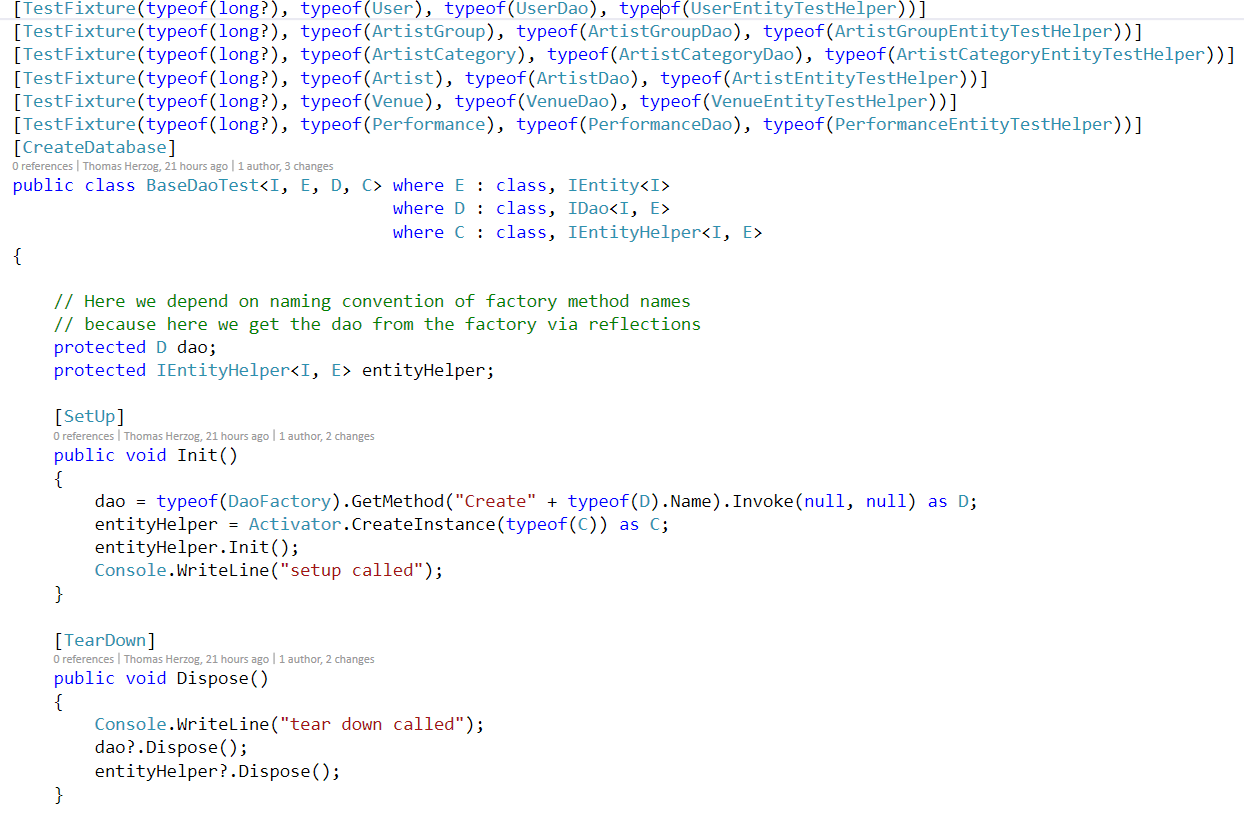
\includegraphics[scale=0.65]{\imagesRoot/basedaotest_screenshot.PNG}
	\caption
	{Ausschnitt aus der Testklasse \emph{BaseDaoTest}}
\end{figure}

\subsection{Ausbaustufe 2 (Commander)}
Folgender Teil dokumentiert die zweite Ausbaustufe des Projektes \emph{UFO} in dem die Administration mit WPF implementiert werden sollte.\\\\
Folgende Projekte wurden der Solution hinzugefügt.
\begin{enumerate}
	\item\emph{UFO.Commander.ServiceApi}\\
	Diese Projekt enthält die Schnittstellen Spezifikation für den Service Layer.
	\item\emph{UFO.Commander.Service.Impl}\\
	Dieses Projekt enthält die Implementierungen der Service Schnittstellen Spezifikationen
	\item\emph{UFO.Commander.Wpf.Administration}\\
	Dieses Projekt enthält die WPF Anwendung, die die Administration abbildet.
\end{enumerate}
\ \\
Des Weiteren wurde der Wurzelnamensraum auf \emph{UFO} beschränkt unter dem jetzt alle Projekte liegen.
\subsubsection{Mögliche Probleme}
Mir ist aufgefallen dass Code im statischen Kontext beim Visual Designer zu Problemen geführt hat, da dieser anscheinend evaluiert wird. Sollten Sie also auf Probleme stoßen so liegt es an folgender Klasse \emph{UFO.Commander.Service.Api.Base.ServiceFactory}.
\newline\newline
Des Weiteren viel mir auf das MySql anscheinend in meiner Version bei einem Prefix diesen nicht in das ResultSet übernimmt. Also eine Query folgendermaßen aussehen könnte.\newline
\emph{SELECT artist.*, venue.* FROM ...} ein Result liefert wie \emph{id, name, id, name}. Sollten Sie eine neuere Version als \emph{5.6.20} könnte dies auf der Performance View Probleme verursachen, da ich davon ausgehe dass diese Verhalten auftritt. 
\subsubsection{Klassenhierarchien}
Folgender Teil der Dokumentation dokumentiert die definierten Klassenhierarchien der WPF Anwendung und des Service Layers.
\newpage
\emph{\textbf{IService}}\\
Folgendes Klassendiagramm zeigt die Hierarchie des Interfaces \emph{IService}, welche die Wurzel aller Service Interfaces darstellt und \emph{IDisposable} erweitert. Somit ist jeder abgeleiteter Service dazu gezwungen die Methode \emph{Dispose} zu implementieren um dort seine gebundenen Ressourcen freizugeben. Des Weiteren wurde eine Basisklasse namens \emph{BaseService} eingeführt, welche die Datenbankverbindung und Transaktionsmethoden implementiert, sodass die abgeleitet Klassen diese Nutzen können.
\begin{figure}[h]
	\centering
	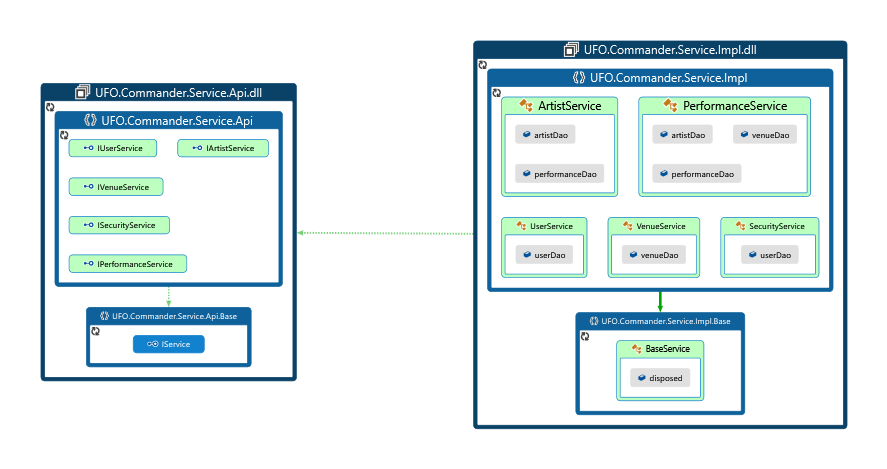
\includegraphics[scale=0.8]{\imagesRoot/iservice_map.PNG}
	\caption
	{Basis Interface für Service Interfaces und Implementierungen}
\end{figure}
\ \\
Alle Services bekommen in Ihrem Konstruktor eine \emph{DbConnection} Instanz übergeben, da alle verwendeten \emph{DAO} Implementierungen dieselbe Datenbank Verbindung nutzen müssen, damit alle sich in derselben Transaktion bewegen.

\newpage
\textbf{\emph{ITabModel}}\\
Folgendes Klassendiagramm zeigt die Hierarchien des Interfaces \emph{ITabModel}, die Operationen definiert, die von der Klasse \emph{TabController} verwendet werden. Die Klasse \emph{TabController} wurde eingeführt um \emph{ITabModel} Instanzen zu initialisieren und beim Wechseln eines Tab aufzuräumen.
\begin{figure}[h]
	\centering
	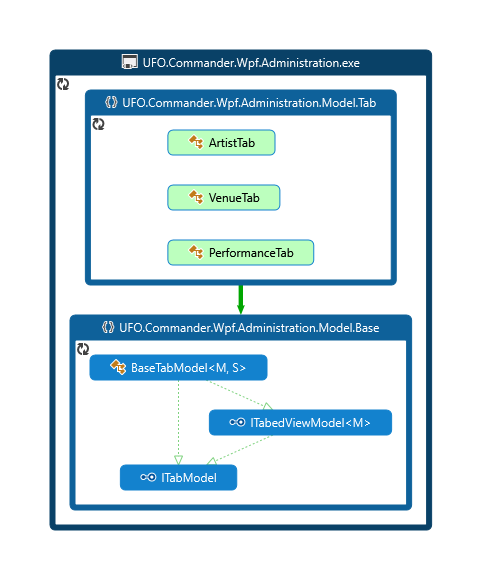
\includegraphics[scale=0.8]{\imagesRoot/basetabmodel_map.PNG}
	\caption
	{Basis Interface für Tab-Model Implementierungen}
\end{figure}
\ \\
Das Interface \emph{ITabedViewModel} definiert die Struktur der Implementierten Tab-Klassen, somit verhält sich jeder Tab gleichermaßen und kann beliebig erweitert werden, je nach seinem View-Content.

\newpage
\textbf{\emph{BasePropertyChangeViewModel}}\\
Folgendes Klassendiagramm zeigt die Hierarchien der Basisklasse \emph{BasePropertyChangeViewModel}, die die Wurzelklasse aller implementierten \emph{View-Models} darstellt, da es immer mindesten einen Property gibt der diesen Event benötigt. Des Weiteren wurde die Klasse \emph{BaseValidationViewModel} eingeführt, die die erste Ableitung von \emph{BasePropertyChangeViewModel} darstellt und die Logik für die Validierung über \emph{System.ComponentModel.DataAnnotations} realisiert. Von dieser Klasse erbt die Basisklasse \emph{BaseEntityViewModel}, die als Wrapper für ViewModels verwendet wird, die eine \emph{IEntity} Instanz für die View wrappen.
\begin{figure}[h]
	\centering
	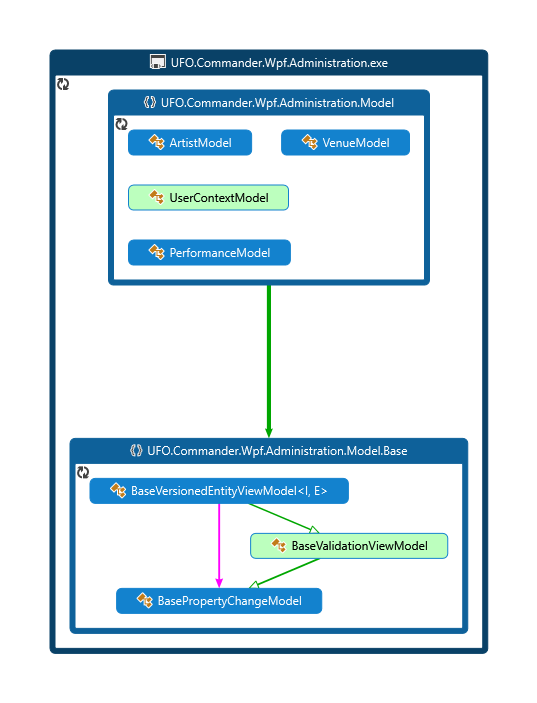
\includegraphics[scale=0.8]{\imagesRoot/viewmodelinheritance_map.PNG}
	\caption
	{Basisklasse für View-Models}
\end{figure}
\ \\
Die Klasse \emph{UserContextModel} wurde eingeführt um einen eingeloggten Benutzer zu repräsentieren und wird als statischer Property der Klasse \emph{App} definiert, da es nur einen eingeloggten Benutzer pro gestarteter Anwendung geben kann. Alle Klassen, die auf den UserContext angewiesen sind müssen die Instanz der Klasse \emph{App} verwenden.

\newpage
\textbf{\emph{SimpleObjectModel}}\\
Folgendes Klassendiagramm zeigt die Hierarchien der Klasse \emph{SimpleObjectModel}, die eingeführt wurde um in Listen, Comboboxen und dergleichen Entitäten für die Darstellung zu halten. Die Controls verwenden Konverter, in denen aus der String Repräsentation wieder in die Entität konvertiert wird. Diese Klasse hält hierbei eine Object Instanz (z.B.: Artist) und den anzuzeigenden Label. In den Konvertern wird eine Instanz \emph{SimpleObjectModel} aus dem zu verwaltenden Objekt erzeugt und visa versa.
\begin{figure}[h]
	\centering
	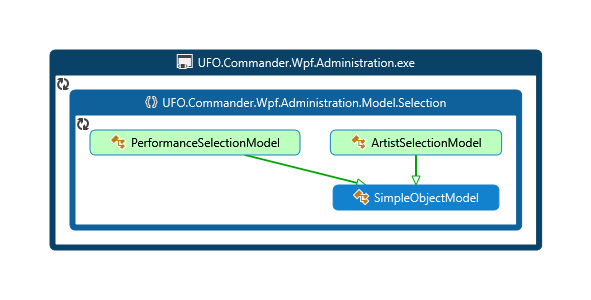
\includegraphics[scale=0.8]{\imagesRoot/simpleobjectmodel_map.PNG}
	\caption
	{Klasse für Controls mit Konverter}
\end{figure}
\ \\
Die beiden abgeleitet Klassen erweitern hierbei die Klasse \emph{SimpleObjectModel} um spezifische Attribute, die in den Controls verwendet werden.

\newpage
\textbf{\emph{IConverter}}\\
Folgendes Klassendiagramm zeigt die Hierarchien der Klasse \emph{IConverter}.
\begin{figure}[h]
	\centering
	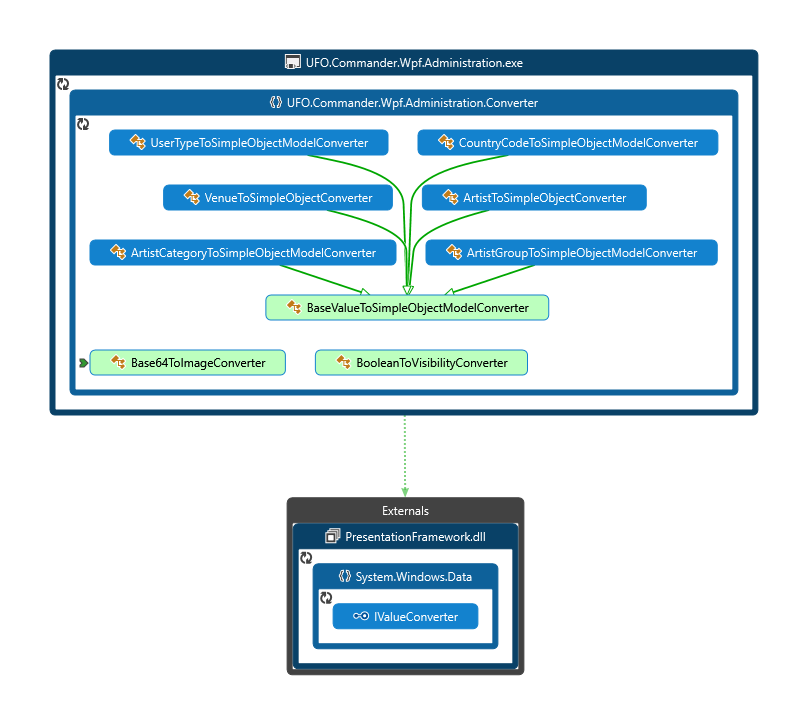
\includegraphics[scale=0.8]{\imagesRoot/iconverter_map.PNG}
	\caption
	{Konverter Hierarchie}
\end{figure}
\ \\
Die Klasse \emph{BaseValueToSimpleObjectConverter} stellt die Basisklasse aller Konverter dar, die Instanzen von \emph{SimpleObjectModel} konvertieren. In diese Klasse wurden alle gemeinsamen Funktionalitäten wie 
\begin{enumerate}
	\item\emph{Typ-Prüfung}\\
	Es wird geprüft ob der Typ des übergebenen Value dem erwarteten Typ entspricht
	\item\emph{ConvertBack}\\
	Da hier nur Instanzen von \emph{SimpleObjectModel} konvertiert werden kann diese Methoden in einer Basisklasse implementiert werden, da hier nur auf den Property \emph{Data} zugegriffen wird.
\end{enumerate}
\ \\
Es wurden auch Konverter für die Visibility (true=Visibility.VISIBILE, false=Visibility.HIDDEN) und zum dekodieren von Base64 Strings in Image Instanzen eingeführt.

\newpage
\subsubsection{WPF Struktur}
Folgende Abbildung zeigt wie die Views innerhalb des Projektes strukturiert wurden.
\begin{figure}[h]
	\centering
	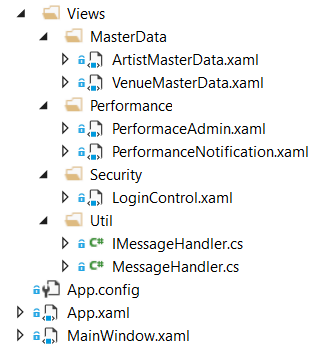
\includegraphics[scale=0.8]{\imagesRoot/viewfolderstructure.PNG}
	\caption
	{Verzeichnisstruktur der Views innerhalb des Projektes}
\end{figure}
\ \\
Bis auf die \emph{App.xaml} und \emph{MainView.xaml} wurden alle Views innerhalb eines Verzeichnis names \emph{Views} gebündelt wobei hierbei eine Trennung zwischen den einzelnen Typen der Views duchgeführt wurde.
\begin{enumerate}
	\item\emph{MasterData}\\
	Alle Views für dier Verwaltung der Stammdaten
	\item\emph{Performance}\\
	Alle Views für die Verwaltung des Festivalprogramms
	\item\emph{Security}\\
	Die Login-View
	\item\emph{Util}\\
	Utility Klassen um innerhalb von View-Models mit der View zu interagieren ohne Referenzen auf WPF Namespaces verwenden zu müssen.
\end{enumerate}
\ \\
Alle diese Views sind als UserControls implementiert worden und werden innerhalb von \emph{MainView.xaml} verwendet (außer PerformanceNotification.xaml), die diese UserControls in einem Tab-Control als DataTemplate für die verschiedene Typen der Tab-Models definiert.
\newline
\newpage
Folgende Abbildung zeigt die eingeführte Verzeichnisstruktur um die WPF-Ressourcen innerhalb diese Projektes zu strukturieren.
\begin{figure}[h]
	\centering
	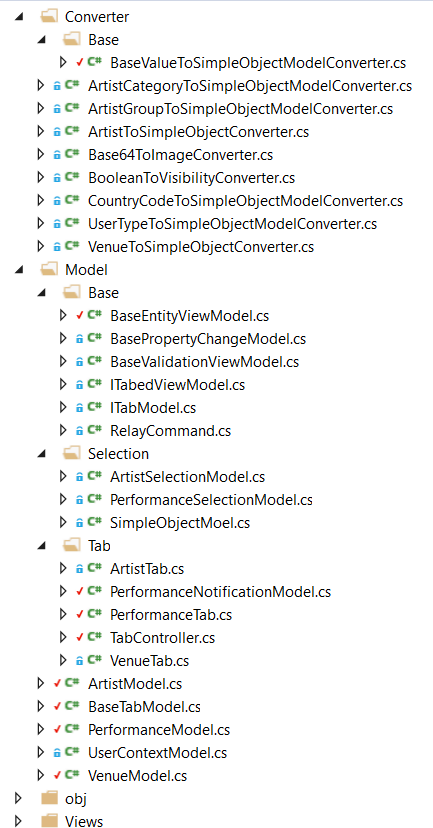
\includegraphics[scale=0.8]{\imagesRoot/wpffolderstrukture.PNG}
	\caption
	{Verzeichnisstruktur der WPF-Ressourcen}
\end{figure}
\ \\
Die jeweiligen Base-Verzeichisse beinhalten die eingeführten Basisklassen für den jeweiligen Kontext (z.B.: Converter, Models, ...).

\newpage
\subsubsection{Benutzerdokumentation}
Folgend ist die Benutzerdokumentation der WPF-Anwendung \emph{Commander} angeführt.
\newline
\newline
\textbf{Login}\newline
Die Administration benötigt einen Login bevor mit Ihr interagiert werden kann. Dazu müssen Sie als Benutzer angelegt worden sein.
\newline
\begin{figure}[h]
	\centering
	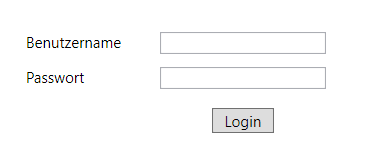
\includegraphics[scale=0.5]{\imagesRoot/view_login.PNG}
	\caption
	{Login nach Start der Anwendung}
\end{figure}
\ \newline
Es wurden keine Beschränkungen beim Login eingeführt, was bedeutet Ihr Zugang wird nach mehrmaligen Fehlversuchen gesperrt.
\newline
\newline
\emph{Mögliche Fehler}
\newline
\newline
Wenn Sie nachdem Start der Anwendung folgende Fehlermeldung erhalten, prüfen Sie bitte ob Sie auf die Datenbank zugreifen können.
\begin{enumerate}
	\item\emph{Fehlende Datenbankverbindung}
	\newline
	Sollten sie keine Datenbankverbindung habe so erhalten Sie folgende Fehlermeldung nach dem Sie die Anwendung gestartet haben. In diesem Fall können Sie sich nicht einloggen.
	\begin{figure}[h]
	\centering
	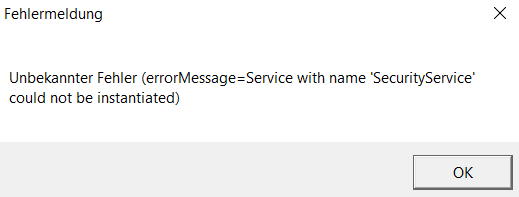
\includegraphics[scale=0.5]{\imagesRoot/view_error_start_app.PNG}
	\caption
	{Fehlermeldung keine Datenbankverbindung}
\end{figure}
\item\emph{Login fehlgeschlagen}
\newline
Wenn Sie ein falsches Passwort eingeben erhalten Sie folgende Fehlermeldung
\begin{figure}[h]
	\centering
	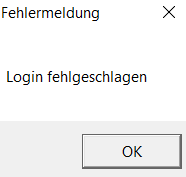
\includegraphics[scale=0.5]{\imagesRoot/view_error_login_failed.PNG}
	\caption
	{Fehlermeldung Login fehlgeschlagen}
\end{figure}
\end{enumerate}
\ \newpage
\parindent0pt{\textbf{Artistenverwaltung}}
\newline
Nachdem Sie sich erfolgreich eingeloggt haben starten Sie mit der Ansicht der Artistenverwaltung, wo Sie die Stammdaten der Artisten verwalten können.
\begin{figure}[h]
	\centering
	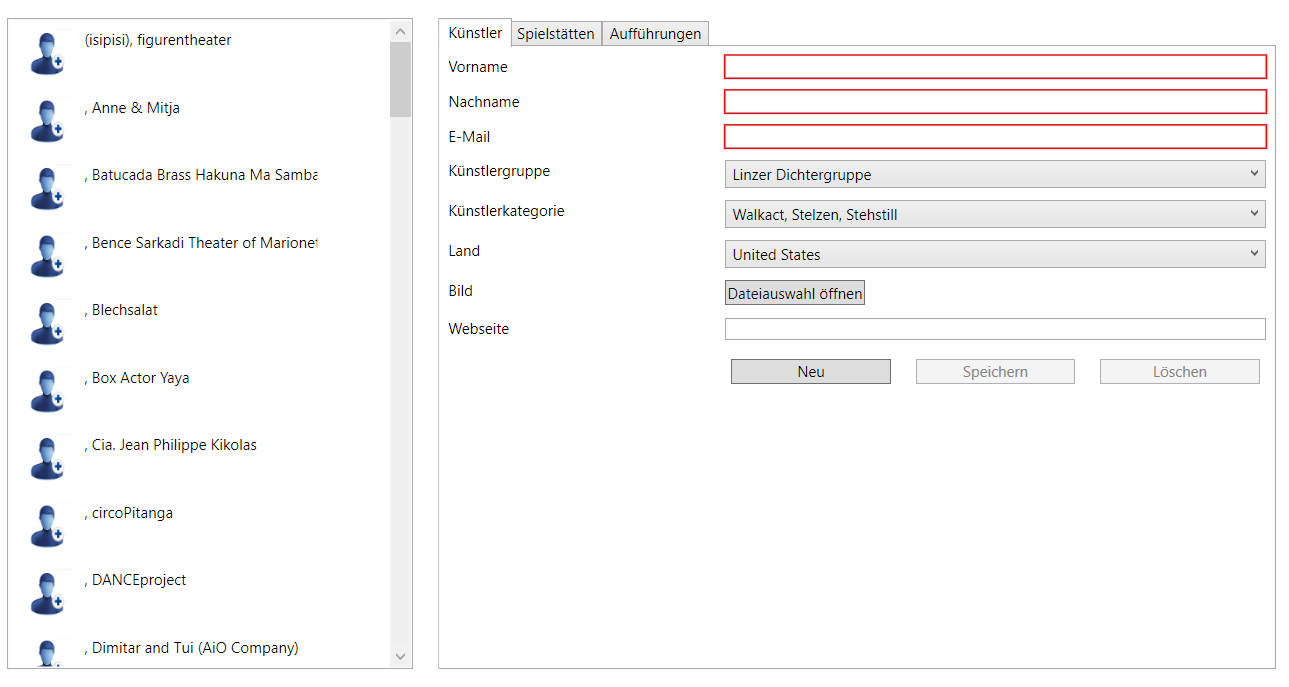
\includegraphics[scale=0.5]{\imagesRoot/view_artist.PNG}
	\caption
	{Stammdatenverwaltung der Artisten}
\end{figure}
\ \newline 
Alle Ansichten sind nachdem selben Schema aufgebaut. Linker Hand sehen Sie die Auswahl der bereits existierenden Einträge - in diesem Fall die Artisten - die Sie auswählen und rechter Hand - innerhalb des Tabs - bearbeiten können. Die rot markierten Eingabefelder signalisieren, dass hier Validierungsfehler aufgetreten sind. Wenn Sie mit dem Cursor über ein rot markiertes Eingabefeld kommen wird Ihnen ein Tooltip angezeigt, der Ihnen mitteilt welcher Validierungsfehler aufgetreten ist.
\newline
\newline
Sollten Sie einen Artisten löschen so werden alle in der Zukunft liegenden Aufführungen dieses Artisten ebenfalls gelöscht. Sollten alle Aufführungen gelöscht worden sein, so wird der Artist ebenfalls gelöscht, andererseits wird der Artist als gelöscht markiert. Auf jeden Fall ist der Artist nicht mehr für Sie verfügbar.
\newline
\newpage
\emph{Mögliche Fehler}
\begin{enumerate}
	\item\emph{Bild zu groß}
	\newline
	Sollten Sie ein Bild auswählen, welches die maximal erlaubte Größe überschreitet, dann erhalten Sie folgende Fehlermeldung
	\begin{figure}[h]
	\centering
	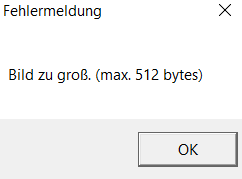
\includegraphics[scale=0.5]{\imagesRoot/view_error_image_too_large.PNG}
	\caption
	{Fehlermeldung Bild zu groß}
\end{figure}
\item\emph{Artist wurde geändert}
\newline
Sollten ein anderer Benutzer den Artisten geändert haben so erhalten Sie folgende Fehlermeldung
	\begin{figure}[h]
	\centering
	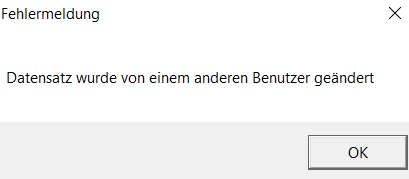
\includegraphics[scale=0.5]{\imagesRoot/view_error_concurrent.PNG}
	\caption
	{Fehlermeldung Artist geändert}
\end{figure}
\item\emph{Artist nicht mehr vorhanden}
\newline
Sollten Sie versuchen einen Artisten zu speichern/löschen und der Artist wurde entweder als gelöscht markiert oder tatsächlich gelöscht, so erhalten Sie folgende Fehlermeldung
	\begin{figure}[h]
	\centering
	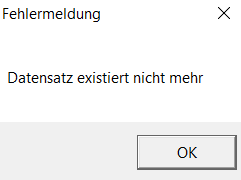
\includegraphics[scale=0.5]{\imagesRoot/view_error_entity_not_existent.PNG}
	\caption
	{Fehlermeldung Artist nicht gefunden}
\end{figure}	
\end{enumerate}
\newpage
\textbf{Spielstätten}
\newline
Auf diesem Tab könne Sie die zur Verfügung stehenden Spielstätten administrieren.
	\begin{figure}[h]
	\centering
	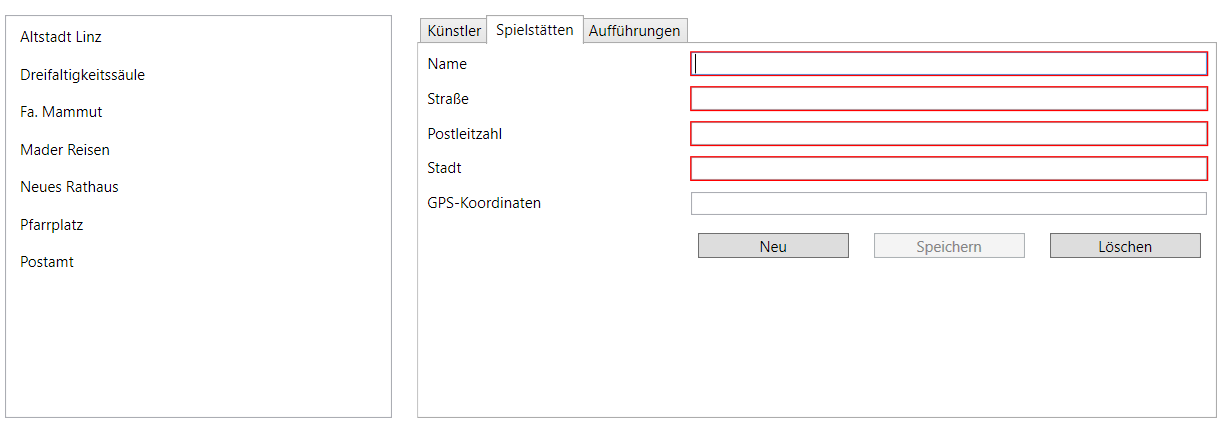
\includegraphics[scale=0.5]{\imagesRoot/view_venue.PNG}
	\caption
	{Stammdatenverwaltung der Spielstätten}
\end{figure}
\ \newline
Bitte stellen Sie sicher das die eingegeben GPS-Koordinaten korrekt sind da hier keine Prüfung auf Korrektheit erfolgt. Sollten Sie GPS-Koordinaten angeben, so können diese in der  Web-Anwendung für Goolge-Maps verwendet werden. Sollten Sie nur die Adressdaten angeben so kann es passieren dass die Position auf Goggle-Maps nicht korrekt angezeigt wird, falls Google diese Adresse nicht kennt oder falsch zuordnet.
\newline
\newline
Sollten bereits Aufführungen an dieser Spielstätte stattfinden, so haben Sie nur mehr die Möglichkeit den Name dieser Spielstätte zu ändern. Bei einem Löschen einer in Verwendung befindlichen Spielstätte wird diese lediglich als gelöscht markiert. In jedem Fall sind gelöschte Spielstätten für Sie nicht mehr verfügbar.
\newline
\newline
\emph{Mögliche Fehler}
\begin{enumerate}
\item\emph{Spielstätte wurde geändert}
\newline
Sollte ein anderer Benutzer die Spielstätte geändert haben so erhalten Sie folgende Fehlermeldung
	\begin{figure}[h]
	\centering
	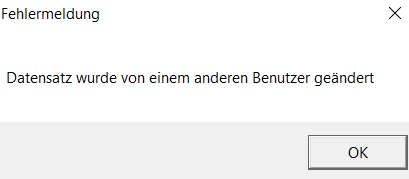
\includegraphics[scale=0.5]{\imagesRoot/view_error_concurrent.PNG}
	\caption
	{Fehlermeldung Spielstätte geändert}
\end{figure}
\item\emph{Spielstätte nicht mehr vorhanden}
\newline
Sollten Sie versuchen eine Spielstätte zu speichern/löschen und die Spielstätte wurde entweder als gelöscht markiert oder tatsächlich gelöscht, so erhalten Sie folgende Fehlermeldung
	\begin{figure}[h]
	\centering
	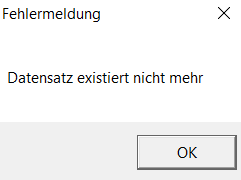
\includegraphics[scale=0.5]{\imagesRoot/view_error_entity_not_existent.PNG}
	\caption
	{Fehlermeldung Spielstätte nicht gefunden}
\end{figure}	
\end{enumerate}
\ \newline
\newpage
\textbf{Aufführungen}
Auf diesem Tab können Sie die Aufführungen verwalten. Diese werden auf die Aufführungstage aufgeteilt und sind in der Auswahl - linker Hand - verfügbar. Hier werden auch Informationen angezeigt wie viele Artisten an wie vielen Spielstätten Aufführungen haben.
	\begin{figure}[h]
	\centering
	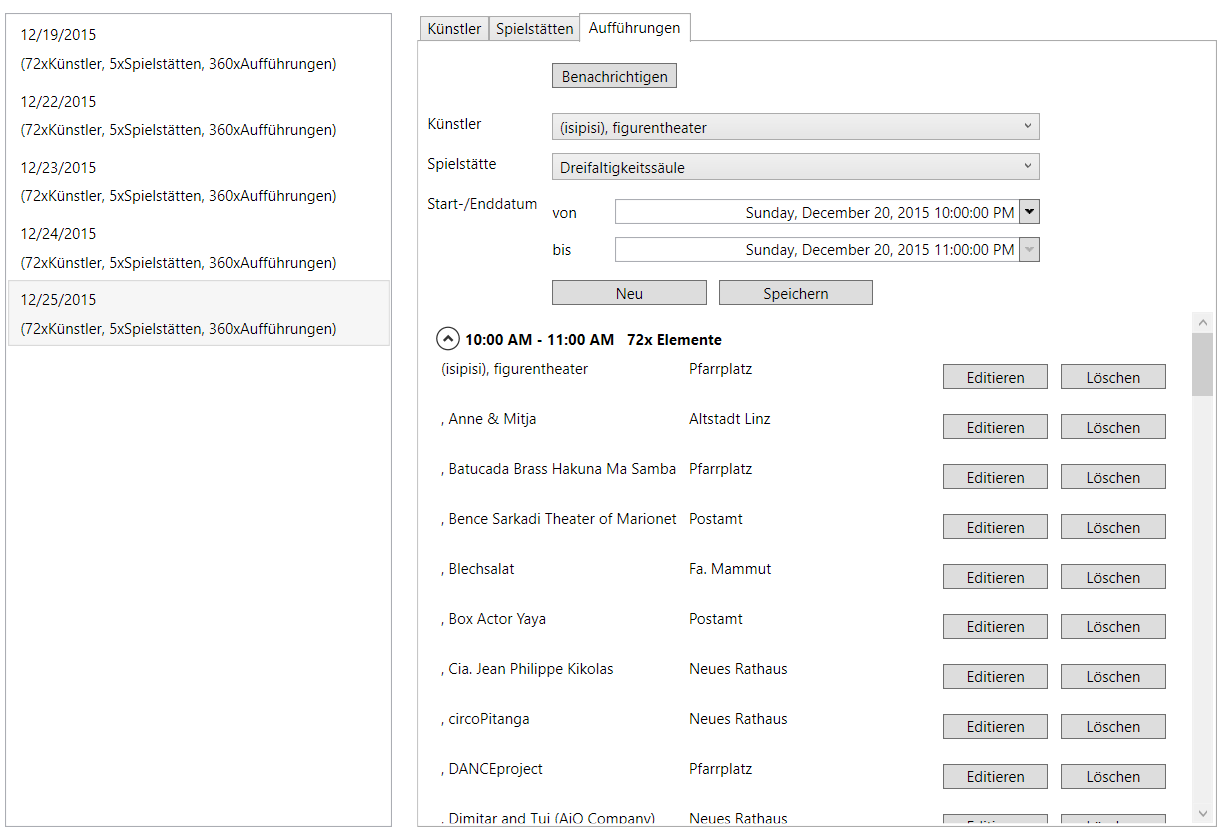
\includegraphics[scale=0.5]{\imagesRoot/view_performance.PNG}
	\caption
	{Festivalverwaltung}
\end{figure}
\ \newline
Nach der Auswahl eines Aufführungstages werden unterhalb des Formulars die Aufführungen geordnet nach der Aufführungszeit, Artistenname und Spielstätte angezeigt. Die Buttons neben den Einträgen signalisieren das diese Einträge änderbar und löschbar sind. Sollten keine Buttons vorhanden sein, so wird diese Aufführung bereits in der Vergangenheit liegen und kann daher weder gelöscht noch geändert werden.
\newline
\newline
Wenn sie auf Editieren klicken so wird das Formular mit den Aufführungsdaten gesetzt und der Button 'Löschen' wird sichtbar. Ansonsten sind die Formularfelder mit Standardwerten befüllt.
\newline
\newline
Wenn Sie den Button 'Benachrichtigen' klicken öffnet sich ein Dialog über den Sie die E-Mail angeben können, die an alle Artisten versendet wird.
	\begin{figure}[h]
	\centering
	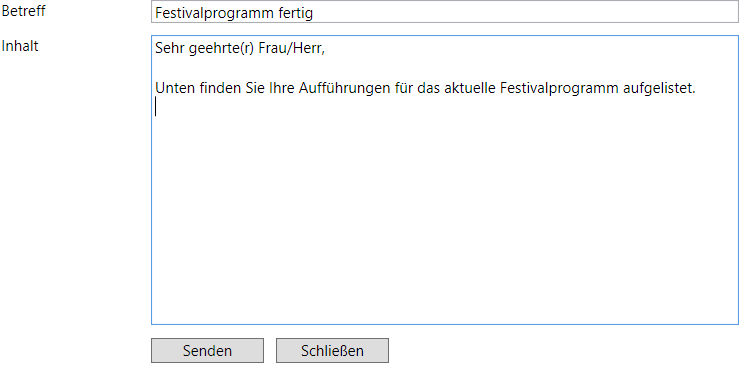
\includegraphics[scale=0.5]{\imagesRoot/view_email_notification.PNG}
	\caption
	{Dialog für E-Mail Benachrichtigungen}
\end{figure}
\ \newline
Diese E-Mail wird an alle Artisten verschickt wobei der E-Mail-Nachricht alle Aufführungen des jeweiligen Artisten angefügt werden.
\newpage
Wenn die E-Mail-Nachrichten versendet wurden erhalten Sie eine Meldung über die Anzahl der versendeten E-Mail-Nachrichten.
	\begin{figure}[h]
	\centering
	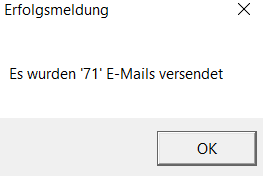
\includegraphics[scale=0.5]{\imagesRoot/view_success_email_sent.PNG}
	\caption
	{Erfolgsmeldung für E-Mail-Versand}
\end{figure}
\ \newline
Sehen Sie hier ein Beispiel für so eine E-Mail Nachricht.
\newline
	\begin{figure}[h]
	\centering
	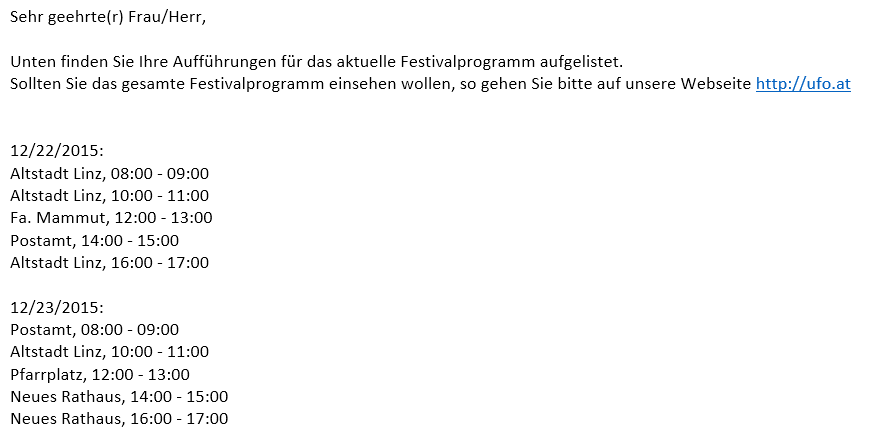
\includegraphics[scale=0.8]{\imagesRoot/sent_email.PNG}
	\caption
	{Generierte E-Mail}
\end{figure}
\ \newline
\newpage
\emph{Mögliche Fehler}
\begin{enumerate}
\item\emph{Aufführung wurde geändert}
\newline
Sollte ein anderer Benutzer die Aufführung geändert haben so erhalten Sie folgende Fehlermeldung
	\begin{figure}[h]
	\centering
	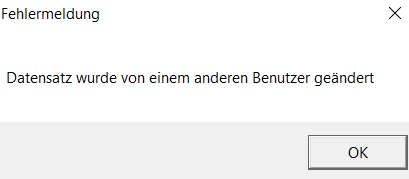
\includegraphics[scale=0.5]{\imagesRoot/view_error_concurrent.PNG}
	\caption
	{Fehlermeldung Spielstätte geändert}
\end{figure}
\item\emph{Aufführung nicht mehr vorhanden}
\newline
Sollten Sie versuchen eine Aufführung zu speichern/löschen und die Aufführung wurde bereits gelöscht so erhalten Sie folgende Fehlermeldung
	\begin{figure}[h]
	\centering
	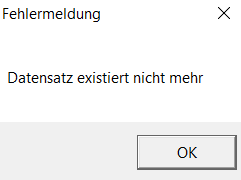
\includegraphics[scale=0.5]{\imagesRoot/view_error_entity_not_existent.PNG}
	\caption
	{Fehlermeldung Spielstätte nicht gefunden}
\end{figure}	
\item\emph{Artist überbucht}
\newline
Sollten Sie versuchen eine Aufführung anzulegen/speichern und der Artist hat bereits eine Aufführung zu diesem Zeitpunkt oder die vordefinierte Pause von 1 Stunde vor und nach einer Aufführung wird unterschritten so erhalten Sie folgende Fehlermeldung
	\begin{figure}[h]
	\centering
	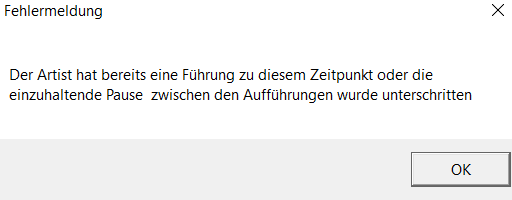
\includegraphics[scale=0.5]{\imagesRoot/view_error_artist_overbooked.PNG}
	\caption
	{Artist überbucht}
\end{figure}
\end{enumerate}
\ \newline
\end{document} 